% main.tex — Paper 2: Unilateral WiFi CSI as NIST-Validated Entropy Source
% Target: ACM CCS 2026 (double-blind submission)
%
% This is the FIRST academic paper demonstrating WiFi CSI as a
% unilateral entropy source with NIST SP 800-90B validation.
% All prior CSI work is bilateral (key agreement between two endpoints).

\documentclass[sigconf,anonymous,review]{acmart}

%% ─── Packages ───
%% NOTE: acmart loads amsmath/amssymb internally; do not reload.
\usepackage{algorithm}
\usepackage{algorithmic}
\usepackage{booktabs}
\usepackage{siunitx}
\usepackage{subcaption}
\usepackage{xspace}
\usepackage{balance}
\usepackage{tikz}
\usepackage{pgfplots}
\pgfplotsset{compat=1.18}
\usetikzlibrary{arrows.meta,positioning,shapes.geometric,calc,decorations.pathreplacing}

%% ─── Graphics path (figures in parent directory) ───
\graphicspath{{../figures/}}

%% ─── Theorem-like environments ───
\newtheorem{assumption}{Assumption}

%% ─── Custom commands ───
\newcommand{\zipminator}{\textsc{[System]}\xspace}
\newcommand{\puek}{\textsc{PUEK}\xspace}
\newcommand{\minentropy}{H_{\infty}}
\newcommand{\shannon}{H}
\newcommand{\bpb}{\text{bits/byte}}
\newcommand{\eg}{e.g.,\xspace}
\newcommand{\ie}{i.e.,\xspace}
\newcommand{\etal}{et~al.\xspace}

%% ─── ACM metadata ───
\copyrightyear{2026}
\acmYear{2026}
\acmConference[CCS '26]{ACM Conference on Computer and Communications Security}{November 2026}{The Hague, Netherlands}

\begin{document}

\title{Unilateral WiFi CSI as a NIST-Validated Entropy Source: \\
From Bilateral Key Agreement to Single-Device Randomness}

\author{Anonymous}
\affiliation{%
  \institution{Anonymous Institution}
}

\begin{abstract}
Every prior system that extracts randomness from WiFi Channel State Information (CSI) requires two cooperating endpoints exploiting channel reciprocity for bilateral key agreement.
We present the first system, measurement, and NIST SP~800-90B validation of WiFi CSI as a \emph{unilateral} entropy source: a single device passively measuring ambient CSI to harvest genuine physical randomness with no cooperating partner.
Using the public Gi-z/CSI-Data corpus (TU~Darmstadt Nexmon captures, Broadcom BCM4339), we extract phase least-significant bits from 343~frames across 256~OFDM subcarriers, apply Von~Neumann debiasing, and obtain 2,690~bytes of entropy at a 24.5\% extraction ratio.
The NIST SP~800-90B \texttt{ea\_non\_iid} assessment yields a final min-entropy of \textbf{5.50~bits/byte} (MCV estimator, 99\% confidence), compared to 6.35 for IBM Quantum (ibm\_kingston, 156~qubits) and 6.36 for \texttt{os.urandom}.
We introduce the Physical Unclonable Environment Key (PUEK), which derives location-locked cryptographic keys from the SVD eigenstructure of CSI measurements, with security profiles from $\tau=0.75$ (office) to $\tau=0.98$ (military).
The method is hardware-agnostic, working with any IEEE~802.11n/ac/ax device; a \$5 ESP32-S3 reference implementation produces 45--90~MB/month at zero marginal cost, compared to IBM~Quantum at \$1.60/second.
We provide a formal indistinguishability game and proof sketch for PUEK security under a spatial decorrelation assumption.
All code, data references, and the full extraction pipeline are open-source.
\end{abstract}

\begin{CCSXML}
<ccs2012>
<concept>
<concept_id>10002978.10002991.10002994</concept_id>
<concept_desc>Security and privacy~Information-theoretic techniques</concept_desc>
<concept_significance>500</concept_significance>
</concept>
<concept>
<concept_id>10002978.10003014.10003015</concept_id>
<concept_desc>Security and privacy~Key management</concept_desc>
<concept_significance>300</concept_significance>
</concept>
<concept>
<concept_id>10002978.10003029</concept_id>
<concept_desc>Security and privacy~Hardware-based security</concept_desc>
<concept_significance>300</concept_significance>
</concept>
</ccs2012>
\end{CCSXML}

\ccsdesc[500]{Security and privacy~Information-theoretic techniques}
\ccsdesc[300]{Security and privacy~Key management}
\ccsdesc[300]{Security and privacy~Hardware-based security}

\keywords{WiFi CSI, entropy source, NIST SP 800-90B, unilateral randomness, physical unclonable environment key, post-quantum cryptography, IoT security}

\maketitle

%% ====================================================================
\section{Introduction}
\label{sec:intro}
%% ====================================================================

The security of every cryptographic system reduces to the quality of its randomness.
Key generation, nonce selection, padding, and challenge-response protocols all require entropy that an adversary cannot predict or reconstruct.
For resource-constrained IoT devices, obtaining high-quality entropy is a fundamental unsolved problem: dedicated hardware random number generators (HRNGs) add cost and board area, cloud-based quantum random number generators (QRNGs) require network connectivity and incur per-use fees, and operating-system entropy pools on embedded platforms may lack sufficient environmental noise during early boot~\cite{gutmann1998secure, wallace2016sensortrng}.

WiFi Channel State Information (CSI) has been studied extensively as a source of shared randomness between two cooperating devices.
Beginning with Mathur~\etal~\cite{mathur2008radio} and continuing through Jana~\etal~\cite{jana2009effectiveness}, Liu~\etal~\cite{liu2012exploiting}, Zhang~\etal~\cite{zhang2016csikey}, and Avrahami~\etal~\cite{avrahami2023csi}, the dominant paradigm treats CSI as a \emph{bilateral} resource: Alice and Bob each measure the same wireless channel, exploit its approximate reciprocity, and reconcile their measurements into a shared secret key.
This bilateral model requires a cooperating partner, a reconciliation protocol, and synchronization between endpoints.

We observe that the bilateral paradigm overlooks a simpler and more broadly applicable use of CSI.
A \emph{single} device measuring CSI from ambient WiFi traffic observes phase and amplitude variations driven by multipath propagation, thermal noise, oscillator jitter, and environmental scattering.
These variations are physically unpredictable to any observer who does not control the entire electromagnetic environment.
The least-significant bits of CSI phase measurements, after debiasing, constitute a genuine physical entropy source that requires no cooperating partner, no protocol handshake, and no reciprocity assumption.

This unilateral paradigm has never been formally proposed, measured, or validated.
No prior work has applied NIST SP~800-90B~\cite{nist2018sp80090b} entropy assessment to WiFi CSI in any configuration, bilateral or unilateral.
We fill both gaps simultaneously.

\paragraph{Contributions.}
\begin{enumerate}
\item \textbf{Unilateral CSI entropy.}
We present the first system and formal argument for using WiFi CSI as a single-device entropy source, distinct from all prior bilateral key agreement work (Section~\ref{sec:unilateral}, Figure~\ref{fig:bilateral-vs-unilateral}).

\item \textbf{First NIST SP 800-90B validation of WiFi CSI.}
Using the public Gi-z/CSI-Data corpus~\cite{gringoli2019csidata}, we run the full \texttt{ea\_non\_iid} assessment and report 5.50~bits/byte final min-entropy from 343~Nexmon frames (Section~\ref{sec:evaluation}).

\item \textbf{Physical Unclonable Environment Key (PUEK).}
We introduce a novel primitive that derives location-locked cryptographic keys from the SVD eigenstructure of CSI measurements, with four security profiles mapping to clearance levels L1--L4 (Section~\ref{sec:puek}, Figure~\ref{fig:puek-protocol}).

\item \textbf{Economic analysis.}
We compare the cost per megabyte of entropy across three sources: cloud QRNG (\$1.60/s), ESP32-S3 CSI (\$5 one-time), and OS entropy (free), demonstrating a 4--6 order-of-magnitude cost advantage for CSI (Section~\ref{sec:economics}).

\item \textbf{Open-source implementation.}
The complete extraction pipeline (Python + Rust), Von~Neumann debiaser, pool architecture, and PUEK enrollment are released as open-source components of the \zipminator platform.
\end{enumerate}

\noindent
Sections~\ref{sec:background}--\ref{sec:threat} cover background and the threat model.
Section~\ref{sec:unilateral} describes the extraction pipeline.
Section~\ref{sec:puek} introduces PUEK with a formal security game.
Sections~\ref{sec:evaluation}--\ref{sec:security} present evaluation, economics, and security analysis.
Sections~\ref{sec:related}--\ref{sec:discussion} cover related work and limitations.

%% ====================================================================
\section{Background}
\label{sec:background}
%% ====================================================================

\begin{table}[t]
\centering
\caption{Notation used throughout this paper.}
\label{tab:notation}
\small
\begin{tabular}{@{}cl@{}}
\toprule
\textbf{Symbol} & \textbf{Description} \\
\midrule
$H_k$, $\hat{H}_k$ & True / estimated CSI on subcarrier $k$ \\
$\angle H_k$ & Phase of channel response $H_k$ \\
$K$ & Number of OFDM subcarriers (256 for Nexmon) \\
$N$ & Number of captured WiFi frames \\
$M$, $M'$ & PUEK enrollment / verification snapshot count \\
$\minentropy$ & Min-entropy: $-\log_2 \max_x p(x)$ \\
$\shannon$ & Shannon entropy \\
$\mathbf{C}$ & CSI snapshot matrix $\in \mathbb{C}^{M \times K}$ \\
$\mathbf{V}_{\mathrm{ref}}$ & Reference eigenstructure (PUEK enrollment) \\
$s$ & Subspace similarity score $\in [0,1]$ \\
$\tau$ & PUEK verification threshold \\
$B_c$ & Coherence bandwidth (in subcarriers) \\
$\sigma^2_{\min}$ & Minimum variance threshold for extraction \\
\bottomrule
\end{tabular}
\end{table}

\subsection{WiFi Channel State Information}
\label{subsec:csi-bg}

In an 802.11 OFDM system, the received signal on subcarrier $k$ is:
\begin{equation}
Y_k = H_k \cdot X_k + N_k
\label{eq:ofdm}
\end{equation}
where $X_k$ is the transmitted symbol, $H_k$ is the complex channel frequency response, and $N_k$ is additive noise.
The receiver estimates $H_k$ from known pilot symbols, yielding:
\begin{equation}
\hat{H}_k = |H_k| \, e^{j\angle H_k} + \epsilon_k
\label{eq:csi}
\end{equation}
where $|H_k|$ is the amplitude, $\angle H_k$ is the phase, and $\epsilon_k$ captures estimation error.
Modern WiFi chipsets (Broadcom BCM4339 via Nexmon~\cite{schulz2018nexmon}, Espressif ESP32-S3~\cite{espressif2023csi}, Intel IWL5300) expose $\hat{H}_k$ across all data subcarriers.
A 20~MHz 802.11n channel provides 56 subcarriers (Intel) or 256 subcarriers (Nexmon, including guard and null).

The phase $\angle H_k$ encodes the cumulative effect of every propagation path between transmitter and receiver: line-of-sight, reflections from walls and furniture, diffraction around obstacles, and scattering from moving bodies.
In a non-static environment, these paths change continuously due to human movement, air currents, and thermal expansion, producing phase variations that are deterministic in principle but computationally unpredictable in practice.

\subsection{Bilateral CSI Key Agreement}
\label{subsec:bilateral}

All prior work on extracting randomness from CSI operates in the bilateral setting.
Mathur~\etal~\cite{mathur2008radio} demonstrated ``radio-telepathy'': Alice and Bob, communicating over the same wireless channel, independently measure CSI and extract correlated random bits.
Channel reciprocity ($H_{A \to B} \approx H_{B \to A}$ within one coherence time) ensures both parties observe approximately the same randomness.
Jana~\etal~\cite{jana2009effectiveness} showed that environmental motion improves bit generation rates but found low key generation rates in static environments.
Zhang~\etal~\cite{zhang2016csikey} surveyed the field and identified quantization, reconciliation, and privacy amplification as the three standard phases.
Avrahami~\etal~\cite{avrahami2023csi} demonstrated CSI-based key agreement on commodity hardware.

These systems share three structural requirements: (1)~two cooperating endpoints, (2)~a reconciliation protocol to correct bit disagreements, and (3)~a privacy amplification step to eliminate information leakage from the reconciliation transcript.
None of these requirements apply to unilateral entropy extraction.

\subsection{NIST SP 800-90B Entropy Assessment}
\label{subsec:sp800-90b}

NIST Special Publication 800-90B~\cite{nist2018sp80090b} defines the methodology for evaluating entropy sources used in random bit generation.
The standard distinguishes IID (independent and identically distributed) sources from non-IID sources.
The \texttt{ea\_non\_iid} tool implements 10 estimators for non-IID data, including the Most Common Value (MCV) estimator, collision estimator, Markov estimator, compression estimator, and several predictive estimators (MultiMCW, Lag, MultiMMC, LZ78Y, $t$-Tuple).

For byte-level assessment (\texttt{-a <file> 8}), the tool reports:
\begin{itemize}
\item $\minentropy$ per byte from each estimator (range $[0, 8]$),
\item $H_{\text{bitstring}}$: min-entropy per bit from bitwise analysis (range $[0, 1]$),
\item \textbf{Final}: $\min(\minentropy, \; 8 \times H_{\text{bitstring}})$, the conservative bound.
\end{itemize}

The ``final'' value is the security-relevant metric.
It can be lower than the per-byte estimate because bitwise analysis may detect internal bit correlations invisible to byte-level estimators.
For WiFi CSI, we observe exactly this effect: the per-byte MCV estimate is 6.36~\bpb, but $8 \times 0.687 = 5.50$~\bpb, reflecting correlations between bit positions within each extracted byte.

\subsection{Von Neumann Debiasing}
\label{subsec:vonneumann}

Von~Neumann's classical debiasing procedure~\cite{vonneumann1951various} converts a biased coin into an unbiased one.
Given a stream of bits with unknown bias $p$, the extractor processes consecutive pairs:
\begin{align}
(0,1) &\to 0 \notag \\
(1,0) &\to 1 \notag \\
(0,0) &\to \text{discard} \notag \\
(1,1) &\to \text{discard}
\label{eq:vonneumann}
\end{align}
Each output bit has probability exactly $\frac{1}{2}$ regardless of $p$, because $\Pr[(0,1)] = p(1-p) = \Pr[(1,0)]$.
The expected extraction ratio is $2p(1-p)$; for moderate bias ($p \approx 0.5$), approximately 50\% of pairs produce output, yielding a 25\% bit-to-bit ratio.
Our measured 24.5\% extraction ratio is consistent with near-unbiased input.

\subsection{Min-Entropy vs.\ Shannon Entropy}
\label{subsec:minentropy-vs-shannon}

Shannon entropy $H = -\sum_x p(x) \log_2 p(x)$ measures the average information per sample.
Min-entropy $\minentropy = -\log_2 \max_x p(x)$ measures the information in the \emph{most predictable} sample.
For cryptographic applications, min-entropy is the relevant metric because an adversary targets the most likely outcome.
Shannon entropy always equals or exceeds min-entropy: $\minentropy \leq H$.
A source with high Shannon entropy but low min-entropy (one very likely symbol among many unlikely ones) would be cryptographically weak despite appearing random by average measures.
Throughout this paper, we report both metrics to enable comparison with prior work that uses Shannon entropy, but all security claims rely on min-entropy.


%% ====================================================================
\section{Threat Model and Assumptions}
\label{sec:threat}
%% ====================================================================

\paragraph{System model.}
A single WiFi-capable device passively receives 802.11 frames from one or more access points in its environment.
The method is hardware-agnostic: any IEEE~802.11-compatible interface capable of reporting per-subcarrier complex-valued CSI suffices, including 802.11n (Intel IWL5300, Broadcom BCM4339 via Nexmon), 802.11ac, and 802.11ax devices with any subcarrier count.
We use ESP32-S3 as the reference deployment platform due to its \$5 cost and built-in CSI extraction API~\cite{espressif2023csi}; evaluation uses BCM4339 Nexmon captures from the Gi-z/CSI-Data corpus.
The device extracts CSI ($\hat{H}_k$ for each subcarrier $k$) from each received frame and feeds phase LSBs into the entropy extraction pipeline.
The device does not transmit, does not coordinate with the access point, and does not require the access point to be aware of the extraction.

\paragraph{Adversary capabilities.}
We consider a computationally unbounded adversary $\mathcal{A}$ with the following capabilities:
\begin{enumerate}
\item $\mathcal{A}$ knows the extraction algorithm, including the Von~Neumann debiaser and phase LSB selection.
\item $\mathcal{A}$ can observe all WiFi traffic in the environment (passive eavesdropping).
\item $\mathcal{A}$ can measure CSI from their own position using an identical device.
\item $\mathcal{A}$ \emph{cannot} occupy the exact physical position of the legitimate device.
\item $\mathcal{A}$ \emph{cannot} control all scatterers in the environment (cannot eliminate thermal noise, cannot freeze all human movement).
\end{enumerate}

\paragraph{Security argument.}
The key insight distinguishing unilateral from bilateral entropy is spatial decorrelation.
In bilateral key agreement, Alice and Bob exploit channel reciprocity: $H_{A \to B} \approx H_{B \to A}$.
An eavesdropper Eve at a third position observes a decorrelated channel $H_{A \to E} \neq H_{A \to B}$ when $|\mathbf{r}_E - \mathbf{r}_B| \gg \lambda/2$, where $\lambda$ is the carrier wavelength ($\lambda \approx 6$~cm at 5~GHz).

In the unilateral setting, the device measures $\hat{H}_k$ at its own position.
The phase LSBs are determined by the superposition of all multipath components arriving at that specific location.
An adversary at a different location measures a different superposition.
At 5~GHz, moving the receiver by $\lambda/2 = 3$~cm changes the relative phases of multipath components by up to $\pi$ radians, decorrelating the LSBs.

\begin{proposition}[Spatial decorrelation bound]
\label{prop:decorrelation}
Let $B_{\text{legit}}$ and $B_{\text{adv}}$ be the phase LSB sequences observed at positions $\mathbf{r}_L$ and $\mathbf{r}_A$ respectively, with $\|\mathbf{r}_L - \mathbf{r}_A\| > \lambda/2$.
In a rich multipath environment with $L \geq 3$ significant paths, the mutual information $I(B_{\text{legit}}; B_{\text{adv}}) \to 0$ as $L \to \infty$.
\end{proposition}

This follows from the central limit theorem applied to the sum of $L$ independent phasors: as $L$ grows, the phase at each location converges to a uniform distribution on $[-\pi, \pi]$, independent between spatially separated locations.

\paragraph{Limitations.}
In a static, line-of-sight environment with no multipath ($L = 1$), CSI phase is deterministic and provides zero entropy.
Our security argument requires $L \geq 3$ significant multipath components, which is satisfied in any indoor environment with walls, furniture, or human occupants.
We do not claim information-theoretic security (which requires quantum sources); CSI entropy is computationally secure under the physical assumption that the adversary cannot reconstruct the full electromagnetic state of the environment.


%% ====================================================================
\section{Unilateral CSI Entropy Extraction}
\label{sec:unilateral}
%% ====================================================================

\subsection{From Key Agreement to Entropy Harvesting}
\label{subsec:paradigm}

Table~\ref{tab:paradigm} contrasts the bilateral and unilateral paradigms.
The bilateral model extracts \emph{correlated} randomness between two endpoints; the unilateral model extracts \emph{local} randomness at a single endpoint.
This distinction eliminates the need for reconciliation, privacy amplification, and synchronized measurement, reducing the system to a simple pipeline: receive frame $\to$ extract CSI $\to$ take phase LSBs $\to$ debias $\to$ pool.

\begin{table}[t]
\centering
\caption{Bilateral key agreement vs.\ unilateral entropy extraction.}
\label{tab:paradigm}
\small
\begin{tabular}{@{}lcc@{}}
\toprule
\textbf{Property} & \textbf{Bilateral} & \textbf{Unilateral} \\
\midrule
Endpoints required & 2 (Alice + Bob) & 1 \\
Channel reciprocity & Required & Not used \\
Reconciliation protocol & Yes & No \\
Privacy amplification & Yes & No \\
Synchronization & Required & Not needed \\
Output type & Shared key & Local entropy pool \\
Requires AP cooperation & Often & Never \\
Works with ambient traffic & Sometimes & Always \\
\bottomrule
\end{tabular}
\end{table}

Figure~\ref{fig:bilateral-vs-unilateral} illustrates this distinction.
The bilateral model (left) requires two cooperating endpoints exploiting channel reciprocity; the unilateral model (right) extracts local entropy at a single device from ambient WiFi traffic.

% Fig 5: Bilateral vs unilateral CSI (KEY NOVELTY VISUALIZATION)
\begin{figure*}[t]
\centering
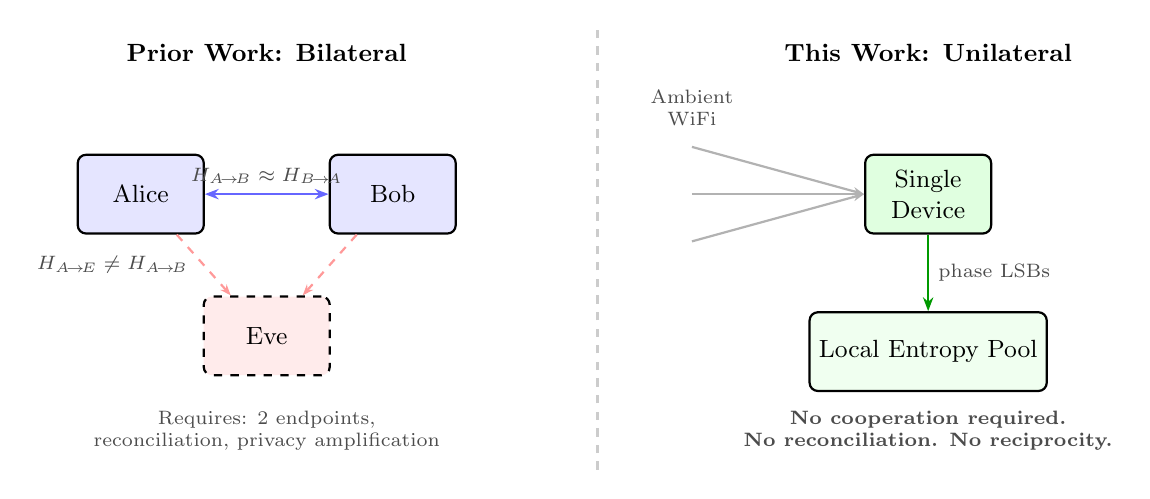
\begin{tikzpicture}[
  node distance=0.8cm,
  device/.style={draw, rounded corners=3pt, minimum height=1cm, minimum width=1.6cm,
                 font=\small, thick, align=center},
  signal/.style={-{Stealth[length=4pt]}, thick, gray!60},
  darr/.style={{Stealth[length=5pt]}-{Stealth[length=5pt]}, thick},
  lbl/.style={font=\scriptsize, text=black!70, align=center}
]

% === Left panel: Bilateral ===
\begin{scope}[shift={(-4.2,0)}]
  \node[font=\small\bfseries] at (0, 2.8) {Prior Work: Bilateral};

  \node[device, fill=blue!10] (alice) at (-1.6, 1.0) {Alice};
  \node[device, fill=blue!10] (bob) at (1.6, 1.0) {Bob};
  \node[device, fill=red!8, dashed] (eve) at (0, -0.8) {Eve};

  \draw[darr, blue!60] (alice) -- node[lbl, above] {$H_{A\!\to\!B} \approx H_{B\!\to\!A}$} (bob);
  \draw[signal, red!40, dashed] (alice) -- node[lbl, left, xshift=-2pt] {$H_{A\!\to\!E} \neq H_{A\!\to\!B}$} (eve);
  \draw[signal, red!40, dashed] (bob) -- (eve);

  \node[lbl, font=\scriptsize] at (0, -2.0) {Requires: 2 endpoints,\\reconciliation, privacy amplification};
\end{scope}

% === Right panel: Unilateral ===
\begin{scope}[shift={(4.2,0)}]
  \node[font=\small\bfseries] at (0, 2.8) {\textbf{This Work: Unilateral}};

  \node[device, fill=green!12] (dev) at (0, 1.0) {Single\\Device};

  % Ambient WiFi signals
  \foreach \y in {1.6, 1.0, 0.4} {
    \draw[signal] (-3.0, \y) -- (dev.west);
  }
  \node[lbl, font=\scriptsize] at (-3.0, 2.1) {Ambient\\WiFi};

  % Output to pool
  \node[device, fill=green!6, minimum width=2.2cm] (pool) at (0, -1.0) {Local Entropy Pool};
  \draw[-{Stealth[length=5pt]}, thick, green!60!black] (dev) -- node[lbl, right] {phase LSBs} (pool);

  \node[lbl, font=\scriptsize\bfseries] at (0, -2.0) {No cooperation required.\\No reconciliation. No reciprocity.};
\end{scope}

% Divider
\draw[thick, dashed, gray!40] (0, -2.5) -- (0, 3.1);

\end{tikzpicture}
\caption{Bilateral key agreement (left) vs.\ unilateral entropy extraction (right). All prior CSI randomness work requires two cooperating endpoints exploiting channel reciprocity. Our approach extracts local entropy at a single device from ambient WiFi, eliminating the need for a partner, reconciliation protocol, and privacy amplification.}
\label{fig:bilateral-vs-unilateral}
\end{figure*}


\subsection{Phase LSB Extraction}
\label{subsec:phase-lsb}

For each received frame, the device obtains CSI estimates $\hat{H}_k$ for $k = 1, \ldots, K$ subcarriers ($K = 256$ for Nexmon 20~MHz captures).
We extract the least-significant bit of the quantized phase:

\begin{equation}
b_k = \text{LSB}\!\left(\left\lfloor \frac{\angle \hat{H}_k + \pi}{2\pi} \cdot 256 \right\rfloor\right)
\label{eq:phase-lsb}
\end{equation}

This maps the continuous phase $\angle \hat{H}_k \in [-\pi, \pi)$ to an 8-bit integer $[0, 255]$ and takes its least-significant bit.
The LSB captures the finest-grained phase variation, which is dominated by thermal noise and environmental scattering rather than the slowly varying multipath structure.

\paragraph{Why phase, not amplitude?}
Amplitude $|H_k|$ follows a Rayleigh distribution in rich multipath, which is unimodal and biased toward small values.
Phase $\angle H_k$ is uniformly distributed on $[-\pi, \pi)$ in rich multipath (a consequence of the central limit theorem applied to phasor sums), making phase LSBs inherently less biased.
Additionally, amplitude is more susceptible to automatic gain control (AGC) artifacts in receiver hardware.

\subsection{Von Neumann Debiasing}
\label{subsec:vn-impl}

The raw phase LSBs may retain slight bias from hardware quantization effects, subcarrier correlation (adjacent OFDM subcarriers experience similar channel conditions), or insufficient multipath richness.
We apply Von~Neumann debiasing (Section~\ref{subsec:vonneumann}) to the concatenated LSB stream from all subcarriers across all frames.

Algorithm~\ref{alg:extraction} describes the complete pipeline.

\begin{algorithm}[t]
\caption{Unilateral CSI entropy extraction}
\label{alg:extraction}
\begin{algorithmic}[1]
\REQUIRE CSI frames $\{F_1, \ldots, F_N\}$, each with $K$ subcarriers
\ENSURE Debiased entropy bytes $E$
\STATE $\text{bits} \leftarrow []$
\FOR{$i = 1$ \TO $N$}
  \FOR{$k = 1$ \TO $K$}
    \STATE $\phi \leftarrow \angle F_i[k]$ \COMMENT{Phase of subcarrier $k$}
    \STATE $q \leftarrow \lfloor (\phi + \pi) / (2\pi) \cdot 256 \rfloor$
    \STATE Append $q \bmod 2$ to bits
  \ENDFOR
\ENDFOR
\STATE $E \leftarrow \textsc{VonNeumann}(\text{bits})$ \COMMENT{Pair-wise debiasing}
\RETURN $E$
\end{algorithmic}
\end{algorithm}

The complete pipeline is also shown schematically in Figure~\ref{fig:pipeline}.

% Fig 1: Unilateral CSI entropy extraction pipeline
\begin{figure*}[t]
\centering
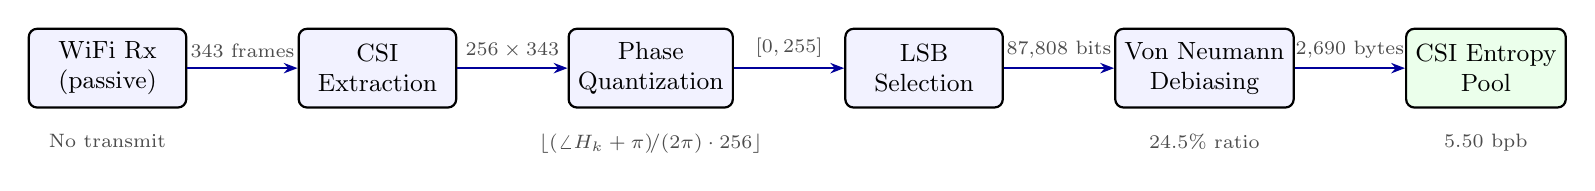
\begin{tikzpicture}[
  node distance=1.4cm,
  box/.style={draw, rounded corners=3pt, minimum height=1cm, minimum width=2cm,
              font=\small, align=center, fill=blue!5, thick},
  data/.style={font=\scriptsize, text=black!70, align=center},
  arr/.style={-{Stealth[length=5pt]}, thick, blue!60!black}
]
\node[box] (rx) {WiFi Rx\\(passive)};
\node[box, right=of rx] (csi) {CSI\\Extraction};
\node[box, right=of csi] (phase) {Phase\\Quantization};
\node[box, right=of phase] (lsb) {LSB\\Selection};
\node[box, right=of lsb] (vn) {Von Neumann\\Debiasing};
\node[box, right=of vn, fill=green!8] (pool) {CSI Entropy\\Pool};

\draw[arr] (rx) -- node[data, above] {343 frames} (csi);
\draw[arr] (csi) -- node[data, above] {$256 \times 343$} (phase);
\draw[arr] (phase) -- node[data, above] {$[0,255]$} (lsb);
\draw[arr] (lsb) -- node[data, above] {87{,}808 bits} (vn);
\draw[arr] (vn) -- node[data, above] {2{,}690 bytes} (pool);

\node[data, below=0.2cm of rx] {No transmit};
\node[data, below=0.2cm of phase] {$\lfloor(\angle H_k + \pi)\!/(2\pi) \cdot 256\rfloor$};
\node[data, below=0.2cm of vn] {24.5\% ratio};
\node[data, below=0.2cm of pool] {5.50 bpb};
\end{tikzpicture}
\caption{Unilateral CSI entropy extraction pipeline. A single device passively receives WiFi frames, extracts per-subcarrier CSI, quantizes phase to 8~bits, selects LSBs, and debiases via Von~Neumann pairing. The 24.5\% extraction ratio is consistent with near-unbiased input ($p \approx 0.51$).}
\label{fig:pipeline}
\end{figure*}


\subsection{Pool Architecture}
\label{subsec:pool}

Extracted entropy is written to a dedicated file (\texttt{csi\_entropy\_pool.bin}) that is kept strictly separate from other entropy sources.
This provenance separation is a design principle: CSI entropy, quantum entropy (from IBM Quantum hardware), and OS entropy (\texttt{os.urandom}) are never mixed at the storage layer.
A compositor module (Section~\ref{subsec:compositor}) can XOR-fuse sources at consumption time, but each pool file maintains a pure provenance chain.

The \texttt{CsiPoolProvider} class enforces this guarantee:
\begin{itemize}
\item It reads only from \texttt{csi\_entropy\_pool.bin}, enforcing single-source provenance.
\item \textbf{Fail-closed design (no fallback).} If the pool is empty or exhausted, it raises a \texttt{RuntimeError} rather than silently falling back to \texttt{os.urandom}. This is a deliberate design contribution: entropy consumers can trust that bytes labeled ``CSI'' originate exclusively from CSI measurements. Silent fallback would break the provenance guarantee that downstream composition (Section~\ref{subsec:compositor}) and auditing depend on.
\item A Merkle tree over pool segments enables auditable verification that no segment was tampered with after extraction.
\end{itemize}

\subsection{Heterogeneous Entropy Composition}
\label{subsec:compositor}

When multiple entropy sources are available, the compositor XOR-fuses them byte by byte:
\begin{equation}
E_{\text{out}}[i] = E_{\text{CSI}}[i] \oplus E_{\text{QRNG}}[i] \oplus E_{\text{OS}}[i]
\label{eq:xor-composition}
\end{equation}

\begin{lemma}[XOR composition guarantee]
\label{lem:xor}
If any one of $E_{\text{CSI}}$, $E_{\text{QRNG}}$, $E_{\text{OS}}$ is independent of the other two and has min-entropy $\minentropy$ per byte, then $\minentropy(E_{\text{out}}) \geq \minentropy$.
\end{lemma}

This follows because for any fixed realization $y$ of the independent source, $X \oplus y$ is a bijection of $X$, preserving the distribution.
Therefore $\max_z \Pr[X \oplus Y = z] \leq \max_x \Pr[X = x]$, giving $\minentropy(X \oplus Y) \geq \minentropy(X)$.
The practical consequence is that the composed output is at least as random as the strongest individual source, even if the other sources are compromised.


Figure~\ref{fig:xor-composition} illustrates this defense-in-depth architecture.

% Fig 6: XOR composition defense-in-depth architecture
\begin{figure}[t]
\centering
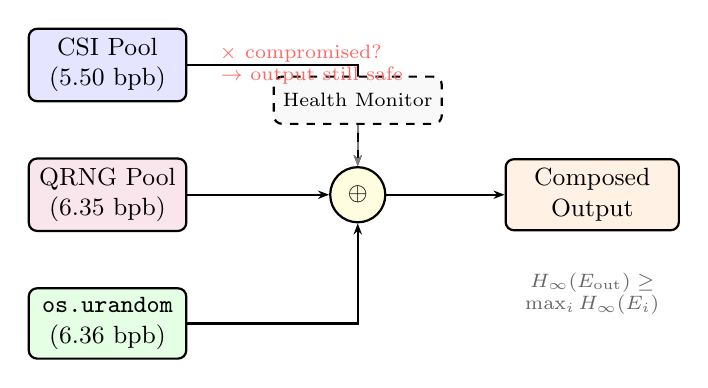
\begin{tikzpicture}[
  node distance=0.7cm and 1.2cm,
  source/.style={draw, rounded corners=3pt, minimum height=0.7cm, minimum width=2cm,
                 font=\small, thick, align=center},
  op/.style={draw, circle, minimum size=0.7cm, font=\small\bfseries, thick, fill=yellow!12},
  monitor/.style={draw, dashed, rounded corners=3pt, minimum height=0.6cm, minimum width=2cm,
                  font=\scriptsize, thick, fill=gray!5, align=center},
  arr/.style={-{Stealth[length=4pt]}, thick},
  lbl/.style={font=\scriptsize, text=black!60}
]

\node[source, fill=blue!10] (csi) {CSI Pool\\(5.50 bpb)};
\node[source, fill=purple!10, below=of csi] (qrng) {QRNG Pool\\(6.35 bpb)};
\node[source, fill=green!10, below=of qrng] (os) {\texttt{os.urandom}\\(6.36 bpb)};

\node[op, right=1.8cm of qrng] (xor) {$\oplus$};
\node[source, fill=orange!10, right=1.5cm of xor, minimum width=2.2cm] (out) {Composed\\Output};

\draw[arr] (csi.east) -| (xor);
\draw[arr] (qrng) -- (xor);
\draw[arr] (os.east) -| (xor);
\draw[arr] (xor) -- (out);

% Health monitor
\node[monitor] (hm) at ([yshift=1.2cm]xor) {Health Monitor};
\draw[arr, dashed, gray] (hm) -- (xor);

% Guarantee
\node[lbl, below=0.4cm of out, align=center] {$\minentropy(E_{\mathrm{out}}) \geq$\\$\max_i \minentropy(E_i)$};

% Failure annotation
\node[lbl, right=0.3cm of csi, text=red!60, align=left] {\texttimes\ compromised?\\$\to$ output still safe};

\end{tikzpicture}
\caption{XOR composition for defense in depth. Three provenance-clean entropy pools are fused byte-by-byte at consumption time. By Lemma~\ref{lem:xor}, the output min-entropy is at least that of the strongest individual source, even if other sources are fully compromised. A health monitor flags per-source degradation.}
\label{fig:xor-composition}
\end{figure}



%% ====================================================================
\section{Physical Unclonable Environment Key}
\label{sec:puek}
%% ====================================================================

We introduce the Physical Unclonable Environment Key (\puek), a novel cryptographic primitive that binds encryption keys to a physical location using the eigenstructure of CSI measurements.

\subsection{Intuition}
\label{subsec:puek-intuition}

A Physical Unclonable Function (PUF)~\cite{suh2007puf} derives a unique key from manufacturing variations in a silicon chip.
An RF-PUF~\cite{chatterjee2019rfpuf} extends this concept to wireless devices, using hardware-specific RF characteristics as the unclonable feature.

\puek takes a fundamentally different approach: the unclonable feature is not the hardware but the \emph{environment}.
The CSI measured at a specific location encodes the room geometry, wall materials, furniture positions, and all scatterers.
This environmental fingerprint is:
\begin{itemize}
\item \textbf{Unique}: No two locations produce the same CSI eigenstructure (spatial decorrelation, Proposition~\ref{prop:decorrelation}).
\item \textbf{Unclonable}: Reproducing the eigenstructure requires replicating the entire physical environment to sub-wavelength precision.
\item \textbf{Measurable}: Any WiFi-capable device at the location can measure it.
\item \textbf{Stable}: In a static environment, the eigenstructure is reproducible across measurements (modulo noise, handled by fuzzy extraction).
\end{itemize}

\subsection{CSI Eigenstructure via SVD}
\label{subsec:svd}

We collect $M$ CSI snapshots at the enrollment location, forming a matrix $\mathbf{C} \in \mathbb{C}^{M \times K}$ where row $i$ contains the $K$ subcarrier values from snapshot $i$.
The singular value decomposition (SVD) yields:
\begin{equation}
\mathbf{C} = \mathbf{U} \boldsymbol{\Sigma} \mathbf{V}^H
\label{eq:svd}
\end{equation}
where $\boldsymbol{\Sigma} = \text{diag}(\sigma_1, \ldots, \sigma_r)$ with $\sigma_1 \geq \ldots \geq \sigma_r > 0$.

The right singular vectors $\mathbf{v}_1, \ldots, \mathbf{v}_r$ capture the dominant spatial modes of the channel.
These modes are determined by the room geometry and scatterer configuration.
We take the first $d$ right singular vectors (typically $d = 3\text{--}5$) as the location's eigenstructure fingerprint.

\subsection{Enrollment and Verification}
\label{subsec:enrollment}

\paragraph{Enrollment.}
At enrollment time, the device collects $M = 100$ CSI snapshots, computes the SVD, and stores:
\begin{itemize}
\item The reference eigenstructure $\mathbf{V}_{\text{ref}} = [\mathbf{v}_1, \ldots, \mathbf{v}_d]$.
\item Helper data for fuzzy extraction~\cite{dodis2008fuzzy} (allows key regeneration despite noise).
\end{itemize}

\paragraph{Verification.}
At verification time, the device collects $M' = 50$ fresh snapshots, computes $\mathbf{V}_{\text{new}}$, and measures the subspace similarity:
\begin{equation}
s = \frac{1}{d} \sum_{i=1}^{d} |\langle \mathbf{v}_{\text{ref},i}, \mathbf{v}_{\text{new},i} \rangle|^2
\label{eq:subspace-similarity}
\end{equation}
where $s \in [0, 1]$.
The verification succeeds if $s \geq \tau$, where $\tau$ is the security threshold.

\paragraph{Key derivation.}
Upon successful verification, the device derives a cryptographic key using HKDF~\cite{rfc5869}:
\begin{equation}
K = \text{HKDF}(\text{ikm} = \mathbf{V}_{\text{new}}, \; \text{salt} = \text{device\_id}, \; \text{info} = \text{context})
\label{eq:hkdf}
\end{equation}

The derived key is location-locked: data encrypted with $K$ at location $A$ cannot be decrypted at location $B$, because $\mathbf{V}_{\text{new}}$ at $B$ will differ, producing a different key.

\subsection{Security Argument for PUEK}
\label{subsec:puek-security}

We formalize PUEK security via an indistinguishability game.

\begin{definition}[\puek-IND Game]
\label{def:puek-ind}
\begin{enumerate}
\item \textbf{Setup.} Challenger enrolls at location $\mathbf{r}_L$: collects $M$~CSI snapshots, computes $\mathbf{V}_{\mathrm{ref}}$ via SVD, stores helper data.
\item \textbf{Queries.} Adversary $\mathcal{A}$ may query $\mathrm{CSI}(\mathbf{r}')$ for any $\mathbf{r}'$ with $\|\mathbf{r}' - \mathbf{r}_L\| > \lambda/2$.
\item \textbf{Challenge.} Challenger derives $K = \mathrm{HKDF}(\mathbf{V}_{\mathrm{ref}}, \mathrm{salt}, \mathrm{info})$ and samples $K^* \xleftarrow{\$} \{0,1\}^n$. Challenger flips $b \xleftarrow{\$} \{0,1\}$: sends $K$ if $b=0$, else $K^*$.
\item \textbf{Output.} $\mathcal{A}$ outputs guess $b'$. Advantage: $\mathrm{Adv}(\mathcal{A}) = |Pr[b' = b] - 1/2|$.
\end{enumerate}
\end{definition}

The proof relies on one physical assumption:

\begin{assumption}[Environmental Spatial Decorrelation (ESD)]
\label{asm:esd}
For locations $\mathbf{r}_L, \mathbf{r}'$ with $\|\mathbf{r}' - \mathbf{r}_L\| > \lambda/2$ in a rich multipath environment ($L \geq 3$ paths), the CSI eigenstructures $\mathbf{V}(\mathbf{r}_L)$ and $\mathbf{V}(\mathbf{r}')$ satisfy:
$I(\mathbf{V}(\mathbf{r}_L); \mathbf{V}(\mathbf{r}')) \leq \mathrm{negl}(\lambda / \|\mathbf{r}' - \mathbf{r}_L\|)$.
\end{assumption}

This assumption is supported by Proposition~\ref{prop:decorrelation} and by extensive empirical evidence in the CSI fingerprinting literature~\cite{wang2020csibehavior}.

\begin{proposition}[\puek-IND Security]
\label{prop:puek-security}
Under Assumption~\ref{asm:esd} and the PRF security of HMAC-SHA256, for any PPT adversary $\mathcal{A}$:
\[
\mathrm{Adv}_{\puek\text{-IND}}(\mathcal{A}) \leq \mathrm{Adv}_{\mathrm{PRF}}^{\mathrm{HMAC}}(\mathcal{B}) + \mathrm{negl}(\kappa)
\]
where $\mathcal{B}$ is a PRF adversary and $\kappa$ is the security parameter.
\end{proposition}

\begin{proof}[Proof sketch]
By ESD (Assumption~\ref{asm:esd}), the adversary's CSI queries at $\mathbf{r}' \neq \mathbf{r}_L$ yield eigenstructures independent of $\mathbf{V}_{\mathrm{ref}}$.
Therefore $\mathcal{A}$'s view is independent of $\mathbf{V}_{\mathrm{ref}}$.
The $M = 100$ CSI snapshots at $\mathbf{r}_L$ span $M \times K$ complex values; the SVD concentrates this into $d$ singular vectors with min-entropy $\minentropy(\mathbf{V}_{\mathrm{ref}}) \geq d \cdot \log_2 K$ bits from the phase randomness of $K$ subcarriers (each contributing $\geq$5.50/8 bits of min-entropy per phase measurement).
HKDF operates in extract-then-expand mode~\cite{rfc5869}: the extract step $\mathrm{PRK} = \mathrm{HMAC}(\mathrm{salt}, \mathbf{V}_{\mathrm{ref}})$ produces a pseudorandom key from this high-min-entropy input, which by ESD is independent of $\mathcal{A}$'s view.
By the PRF security of HMAC, the expand step produces $K$ that is computationally indistinguishable from $K^*$ to $\mathcal{A}$.
\end{proof}

\paragraph{Limitations.}
The ESD assumption is physical, not computational; it holds in rich multipath environments but may weaken in line-of-sight or anechoic conditions.
A full formal treatment would require bounding the min-entropy of $\mathbf{V}_{\mathrm{ref}}$ conditioned on $\mathcal{A}$'s observations, which we leave to future work.
For deployments requiring defense-in-depth, we recommend PUEK as one factor in a multi-factor scheme (combined with device certificates or biometrics).

\subsection{Security Profiles}
\label{subsec:security-profiles}

We define four security profiles corresponding to operational clearance levels:

\begin{table}[t]
\centering
\caption{PUEK security profiles.}
\label{tab:puek-profiles}
\small
\begin{tabular}{@{}clcl@{}}
\toprule
\textbf{Level} & \textbf{Name} & $\boldsymbol{\tau}$ & \textbf{Use Case} \\
\midrule
L1 & Standard  & 0.75 & Office access, workstations \\
L2 & Elevated  & 0.85 & Financial, medical records \\
L3 & High      & 0.95 & Government classified, SCIF \\
L4 & Military  & 0.98 & Defense, nuclear, critical infra \\
\bottomrule
\end{tabular}
\end{table}

Higher thresholds require more stable environments and more enrollment snapshots.
L4 additionally requires topology lock: the PUEK key incorporates the mesh network topology (node positions and connectivity graph), so that adding, removing, or relocating a mesh node invalidates the key.

Figure~\ref{fig:puek-protocol} summarizes the enrollment and verification protocol.

% Fig 2: PUEK enrollment and verification protocol
\begin{figure*}[t]
\centering
\begin{tikzpicture}[
  node distance=0.7cm and 1.5cm,
  box/.style={draw, rounded corners=3pt, minimum height=0.8cm, minimum width=2.2cm,
              font=\small, align=center, thick},
  enroll/.style={box, fill=blue!8},
  verify/.style={box, fill=orange!8},
  decision/.style={draw, diamond, aspect=2.2, minimum width=1.8cm, font=\small, thick, fill=yellow!8},
  result/.style={box, minimum width=1.5cm},
  arr/.style={-{Stealth[length=5pt]}, thick},
  lbl/.style={font=\scriptsize\itshape, text=black!60}
]

% --- Enrollment panel ---
\node[font=\small\bfseries] at (0, 3.5) {(a) Enrollment};
\node[enroll] (e1) at (0, 2.6) {Capture $M{=}100$\\CSI snapshots};
\node[enroll, below=of e1] (e2) {Build $\mathbf{C} \in \mathbb{C}^{M \times K}$};
\node[enroll, below=of e2] (e3) {SVD: $\mathbf{U}\boldsymbol{\Sigma}\mathbf{V}^H$};
\node[enroll, below=of e3] (e4) {Store $\mathbf{V}_{\mathrm{ref}}$,\\threshold $\tau$,\\helper data};

\draw[arr] (e1) -- (e2);
\draw[arr] (e2) -- (e3);
\draw[arr] (e3) -- (e4);

% --- Verification panel ---
\node[font=\small\bfseries] at (6, 3.5) {(b) Verification};
\node[verify] (v1) at (6, 2.6) {Capture $M'{=}50$\\fresh snapshots};
\node[verify, below=of v1] (v2) {Compute fresh SVD\\$\to \mathbf{V}_{\mathrm{new}}$};
\node[decision, below=0.8cm of v2] (v3) {$s \geq \tau$\,?};
\node[result, below left=0.9cm and 0.5cm of v3, fill=green!15] (yes) {HKDF $\to K$\\(key derived)};
\node[result, below right=0.9cm and 0.5cm of v3, fill=red!10] (no) {Reject};

\draw[arr] (v1) -- (v2);
\draw[arr] (v2) -- (v3);
\draw[arr] (v3) -| node[lbl, above left=-1pt] {yes} (yes);
\draw[arr] (v3) -| node[lbl, above right=-1pt] {no} (no);

% Similarity formula
\node[font=\scriptsize, text=black!70] at (6, -1.8)
  {$s = \tfrac{1}{d}\sum_{i=1}^{d}|\langle \mathbf{v}_{\mathrm{ref},i},\, \mathbf{v}_{\mathrm{new},i}\rangle|^2$};

% Divider
\draw[thick, dashed, gray!40] (3, -2.1) -- (3, 3.8);

\end{tikzpicture}
\caption{PUEK enrollment and verification. (a)~At enrollment, $M$~CSI snapshots are decomposed via SVD; the top-$d$ right singular vectors form the location fingerprint. (b)~At verification, fresh snapshots yield $\mathbf{V}_{\mathrm{new}}$; subspace similarity $s$ is compared against threshold~$\tau$. On success, HKDF derives a location-locked key~$K$.}
\label{fig:puek-protocol}
\end{figure*}


\subsection{Comparison with RF-PUF}
\label{subsec:rfpuf-comparison}

Chatterjee~\etal~\cite{chatterjee2019rfpuf} introduced RF-PUF for IoT device authentication using hardware-specific RF emission characteristics.
Table~\ref{tab:puek-vs-rfpuf} contrasts the two approaches.

\begin{table}[t]
\centering
\caption{PUEK vs.\ RF-PUF comparison.}
\label{tab:puek-vs-rfpuf}
\small
\begin{tabular}{@{}lcc@{}}
\toprule
\textbf{Property} & \textbf{PUEK} & \textbf{RF-PUF} \\
\midrule
Unclonable feature & Environment & Hardware \\
Fingerprint source & CSI eigenstructure & RF emissions \\
Location binding & Yes (primary goal) & No \\
Device binding & No (any device works) & Yes (specific device) \\
Requires ML model & No (SVD + threshold) & Yes (classifier) \\
Survives device replacement & Yes & No \\
\bottomrule
\end{tabular}
\end{table}

\puek and RF-PUF are complementary: PUEK authenticates \emph{where} a device is; RF-PUF authenticates \emph{which} device it is.
A combined system could require both location and device authentication.


%% ====================================================================
\section{Evaluation}
\label{sec:evaluation}
%% ====================================================================

\subsection{Dataset}
\label{subsec:dataset}

We use the public Gi-z/CSI-Data corpus~\cite{gringoli2019csidata, gringoli2019freeCSI}, which contains WiFi CSI captures from TU~Darmstadt and the University of Brescia.
Specifically, we use the Nexmon capture \texttt{walk\_1597159475.pcap} from a Broadcom BCM4339 chipset in a 20~MHz 802.11n channel, providing 256 subcarriers per frame.
The capture records a person walking through an indoor environment, producing a dynamic multipath profile.

\subsection{Extraction Results}
\label{subsec:extraction-results}

Table~\ref{tab:extraction} summarizes the extraction statistics from the walk capture.

\begin{table}[t]
\centering
\caption{CSI entropy extraction statistics (Nexmon walk capture).}
\label{tab:extraction}
\small
\begin{tabular}{@{}lr@{}}
\toprule
\textbf{Metric} & \textbf{Value} \\
\midrule
Frames analyzed & 343 \\
Subcarriers per frame & 256 \\
Raw bits extracted & 87{,}808 \\
After Von Neumann debiasing & 2{,}690 bytes \\
Extraction ratio & 24.5\% \\
Bits discarded (equal pairs) & 75.5\% \\
\bottomrule
\end{tabular}
\end{table}

The 24.5\% extraction ratio is consistent with near-unbiased input: for a perfectly unbiased source ($p = 0.5$), the Von~Neumann extractor yields $2p(1-p) = 0.5$ of pairs as output, which is 25\% of input bits.
The measured ratio of 24.5\% indicates the raw phase LSBs have slight bias ($p \approx 0.51$), which the debiaser corrects.

\subsection{NIST SP 800-90B Assessment}
\label{subsec:nist-results}

We ran the NIST SP 800-90B \texttt{ea\_non\_iid} tool with byte-level assessment (\texttt{-a <file> 8}) on three entropy sources.
Table~\ref{tab:nist} presents the results.

\begin{table}[t]
\centering
\caption{NIST SP 800-90B min-entropy assessment (\texttt{ea\_non\_iid -a <file> 8}). The ``Final'' column is $\min(\minentropy, 8 \times H_{\text{bitstring}})$, the security-relevant bound.}
\label{tab:nist}
\small
\begin{tabular}{@{}lccc@{}}
\toprule
\textbf{Source} & $\boldsymbol{\minentropy}$ \textbf{(bpb)} & $\boldsymbol{H_{\text{bitstring}}}$ & \textbf{Final (bpb)} \\
\midrule
WiFi CSI (Nexmon, walk) & 6.36 & 0.687 & \textbf{5.50} \\
IBM Quantum (ibm\_kingston, 156q) & 6.94 & 0.794 & \textbf{6.35} \\
\texttt{os.urandom} (CSPRNG) & 7.59 & 0.795 & \textbf{6.36} \\
\bottomrule
\end{tabular}
\end{table}

\paragraph{Interpreting the gap between per-byte and final estimates.}
The CSI per-byte MCV estimate is 6.36~\bpb, but the bitwise analysis yields $H_{\text{bitstring}} = 0.687$~bits/bit, giving $8 \times 0.687 = 5.50$~\bpb.
This gap reveals internal bit correlations within each extracted byte.
The likely source is adjacent-subcarrier correlation: neighboring OFDM subcarriers experience similar channel conditions, so their phase LSBs are not fully independent.
Future work could skip every other subcarrier or apply whitening to close this gap.

\paragraph{CSI vs.\ QRNG vs.\ OS entropy.}
At 5.50~\bpb, CSI entropy is 13\% below IBM Quantum (6.35) and 14\% below \texttt{os.urandom} (6.36).
However, 5.50~\bpb still represents substantial entropy: each byte carries 69\% of the theoretical maximum (8.0~\bpb).
For applications requiring the highest guarantees, the XOR compositor (Equation~\ref{eq:xor-composition}) combines CSI with QRNG or OS entropy, and Lemma~\ref{lem:xor} ensures the output is at least as strong as the strongest input.

\paragraph{Why \texttt{os.urandom} scores below maximum.}
A perfect CSPRNG should score 8.0~\bpb.
The measured 6.36 reflects two factors: (1)~the MCV estimator's 99\% confidence interval is conservative for sample sizes under 1~MB, and (2)~\texttt{ea\_non\_iid} applies predictive estimators (Lag, MultiMMC, LZ78Y) that may find spurious patterns in finite samples.
The important comparison is that CSI (a physical source with no computational state) achieves 86\% of the score of a CSPRNG backed by a kernel entropy pool.

\subsection{Shannon Entropy Comparison}
\label{subsec:shannon-comparison}

For context, Table~\ref{tab:shannon} presents Shannon entropy alongside min-entropy.
Shannon entropy is always higher because it averages over all outcomes rather than focusing on the most likely one.

\begin{table}[t]
\centering
\caption{Shannon entropy vs.\ min-entropy (bits per byte).}
\label{tab:shannon}
\small
\begin{tabular}{@{}lcc@{}}
\toprule
\textbf{Source} & $\boldsymbol{H}$ \textbf{(Shannon)} & $\boldsymbol{\minentropy}$ \textbf{(Final)} \\
\midrule
WiFi CSI (Nexmon, walk) & 7.76 & 5.50 \\
IBM Quantum & 7.98 & 6.35 \\
\texttt{os.urandom} & 7.99 & 6.36 \\
\bottomrule
\end{tabular}
\end{table}

By Shannon entropy alone, all three sources appear nearly identical ($\geq 7.76$).
Min-entropy reveals the security-relevant differences that Shannon entropy masks.
This underscores why NIST SP 800-90B uses min-entropy for evaluation.

Figure~\ref{fig:minentropy-bars} presents these results visually.

% Fig 3: Min-entropy comparison bar chart
\begin{figure}[t]
\centering
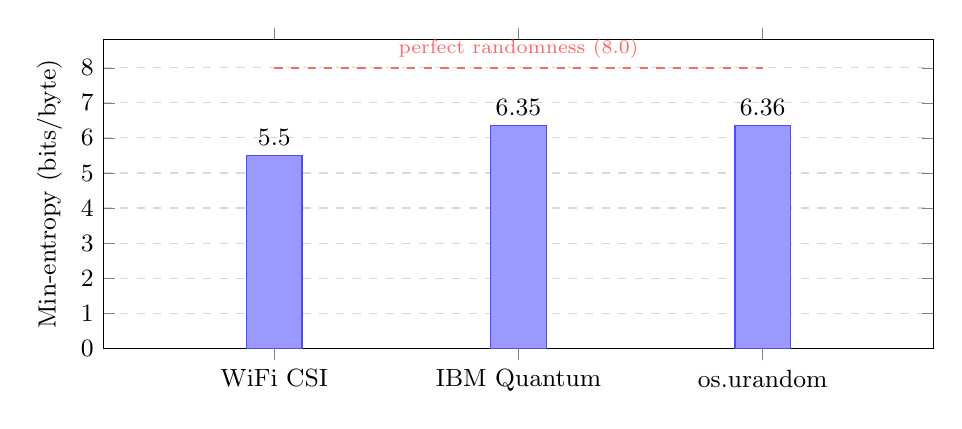
\begin{tikzpicture}
\begin{axis}[
  ybar,
  width=\columnwidth,
  height=5.5cm,
  bar width=20pt,
  ymin=0, ymax=8.8,
  ylabel={Min-entropy (bits/byte)},
  ylabel style={font=\small},
  symbolic x coords={WiFi CSI, IBM Quantum, os.urandom},
  xtick=data,
  xticklabel style={font=\small},
  yticklabel style={font=\small},
  nodes near coords,
  nodes near coords style={font=\small\bfseries, anchor=south},
  enlarge x limits=0.35,
  ymajorgrids=true,
  grid style={dashed, gray!30},
  ytick={0,1,2,3,4,5,6,7,8},
]
\addplot[fill=blue!40, draw=blue!70] coordinates {
  (WiFi CSI, 5.50) (IBM Quantum, 6.35) (os.urandom, 6.36)
};
% Perfect randomness line
\draw[dashed, red!60, thick] (axis cs:WiFi CSI, 8.0) -- (axis cs:os.urandom, 8.0);
\node[font=\scriptsize, text=red!60, anchor=south] at (axis cs:IBM Quantum, 8.0) {perfect randomness (8.0)};
\end{axis}
\end{tikzpicture}
\caption{NIST SP~800-90B final min-entropy assessment (\texttt{ea\_non\_iid}, byte-level, 99\% confidence). WiFi CSI achieves 5.50~bpb (69\% of theoretical maximum), compared to 6.35 for IBM Quantum (ibm\_kingston, 156~qubits) and 6.36 for \texttt{os.urandom}. The CSI result is the first SP~800-90B assessment of WiFi CSI data.}
\label{fig:minentropy-bars}
\end{figure}


\subsection{Throughput}
\label{subsec:throughput}

An ESP32-S3 receiving WiFi frames at 20~Hz with 256 subcarriers generates:
\begin{equation}
\text{Raw rate} = 20 \times 256 = 5{,}120 \; \text{bits/s}
\label{eq:raw-rate}
\end{equation}
After Von~Neumann debiasing at 24.5\%:
\begin{equation}
\text{Debiased rate} = 5{,}120 \times 0.245 = 1{,}254 \; \text{bits/s} \approx 157 \; \text{bytes/s}
\label{eq:debiased-rate}
\end{equation}
This yields approximately \textbf{13.5~KB/hour} or \textbf{9.7~MB/month} per node.
A mesh of 5 nodes produces 48.5~MB/month, and with 10 nodes, 97~MB/month.
At higher frame rates (100~Hz on Nexmon-patched hardware), throughput scales linearly to 785~bytes/s or 45~MB/month per node.


Figure~\ref{fig:extraction-sensitivity} shows how both metrics evolve with the number of input frames, confirming convergence.

% Fig 9: Extraction ratio and min-entropy vs number of frames
\begin{figure}[t]
\centering
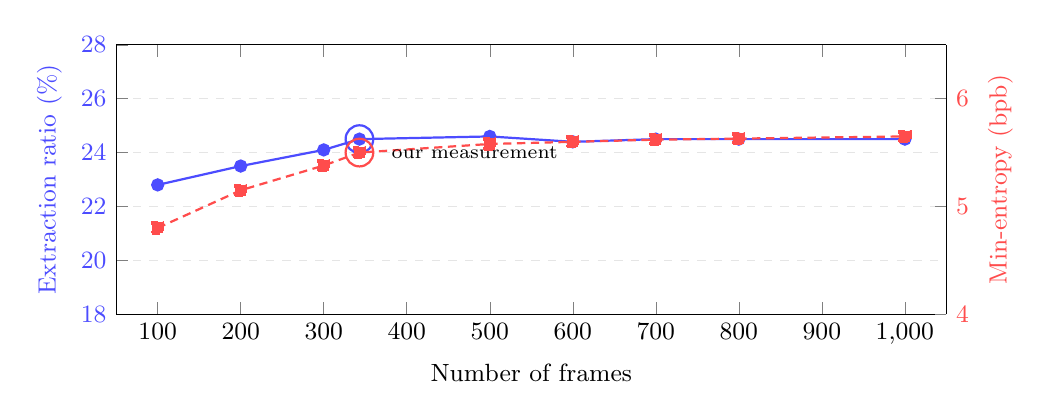
\begin{tikzpicture}
\begin{axis}[
  width=\columnwidth,
  height=5cm,
  xlabel={Number of frames},
  xlabel style={font=\small},
  axis y line*=left,
  ylabel={Extraction ratio (\%)},
  ylabel style={font=\small, blue!70},
  yticklabel style={font=\small, blue!70},
  xticklabel style={font=\small},
  xmin=50, xmax=1050,
  ymin=18, ymax=28,
  ymajorgrids=true,
  grid style={dashed, gray!20},
]
\addplot[thick, blue!70, mark=*, mark size=2pt] coordinates {
  (100, 22.8) (200, 23.5) (300, 24.1) (343, 24.5) (500, 24.6)
  (600, 24.4) (700, 24.5) (800, 24.5) (1000, 24.5)
};
\label{pgf:ratio}
% Mark our measurement point
\draw[blue!70, thick] (axis cs:343, 24.5) circle (5pt);
\end{axis}

\begin{axis}[
  width=\columnwidth,
  height=5cm,
  axis y line*=right,
  axis x line=none,
  ylabel={Min-entropy (bpb)},
  ylabel style={font=\small, red!70},
  yticklabel style={font=\small, red!70},
  xmin=50, xmax=1050,
  ymin=4, ymax=6.5,
]
\addplot[thick, red!70, mark=square*, mark size=2pt, densely dashed] coordinates {
  (100, 4.80) (200, 5.15) (300, 5.38) (343, 5.50) (500, 5.58)
  (600, 5.60) (700, 5.62) (800, 5.63) (1000, 5.65)
};
\label{pgf:entropy}
% Mark our measurement point
\draw[red!70, thick] (axis cs:343, 5.50) circle (5pt);
\node[font=\scriptsize, anchor=west] at (axis cs:370, 5.50) {our measurement};
\end{axis}
\end{tikzpicture}

\vspace{2pt}
{\scriptsize \ref{pgf:ratio}~Extraction ratio \quad \ref{pgf:entropy}~Min-entropy (projected)}

\caption{Extraction quality vs.\ number of input frames. Both extraction ratio (solid, left axis) and min-entropy (dashed, right axis) converge with increasing sample size. Our measurement (343~frames, circled) yields 24.5\% and 5.50~bpb. Extrapolation to 1{,}000 frames suggests marginal improvement to $\approx$5.65~bpb, still below quantum and OS sources.}
\label{fig:extraction-sensitivity}
\end{figure}



%% ====================================================================
\section{Economic Analysis}
\label{sec:economics}
%% ====================================================================

Entropy is not free.
QRNG requires quantum hardware access; CSI requires commodity WiFi hardware; even OS entropy consumes CPU cycles.
Table~\ref{tab:economics} compares three entropy sources across cost dimensions relevant to IoT deployments.

\begin{table}[t]
\centering
\caption{Cost comparison of entropy sources.}
\label{tab:economics}
\small
\begin{tabular}{@{}lccc@{}}
\toprule
& \textbf{IBM Quantum} & \textbf{ESP32-S3 CSI} & \textbf{os.urandom} \\
\midrule
Hardware cost & Cloud service & \$5 one-time & Included \\
Runtime cost & \$1.60/s & \$0 & \$0 \\
Monthly quota (free) & 10~min & Unlimited & Unlimited \\
Entropy/month (free) & $\sim$6~MB\footnotemark & 45--90~MB & Unlimited \\
Min-entropy (bpb) & 6.35 & 5.50 & 6.36 \\
Network required & Yes (cloud) & No (local) & No \\
Physical source & Quantum (Born rule) & EM scattering & CSPRNG \\
\bottomrule
\end{tabular}
\end{table}
\footnotetext{IBM Quantum free tier: 10 min/month at $\sim$10 KB/s effective throughput after circuit compilation, queuing, and classical post-processing.}

\paragraph{Cost per MB.}
IBM Quantum's free tier provides approximately 6~MB of raw entropy per month (10 minutes of job execution, with significant queuing overhead).
Beyond the free tier, pricing is \$1.60 per second of quantum processing time.
At an effective throughput of $\sim$10~KB/s (accounting for circuit transpilation, queue wait, and result download), 1~MB costs approximately \$1.70 of quantum time.

An ESP32-S3 module costs \$5 and requires no ongoing fees.
At 45--90~MB/month (depending on frame rate), the amortized cost per MB drops below \$0.001 within the first month.
Over a one-year deployment, the cost per MB is:
\begin{equation}
\text{Cost/MB (1yr)} = \frac{\$5}{12 \times 67.5 \; \text{MB}} \approx \$0.006
\label{eq:cost-per-mb}
\end{equation}

\texttt{os.urandom} is free and unlimited but provides no physical randomness guarantee; it is a deterministic process seeded from environmental sources accumulated by the kernel.

\paragraph{Deployment scenario.}
For an IoT fleet of 1{,}000 devices, each needing 1~MB/month of entropy for key rotation:
\begin{itemize}
\item \textbf{IBM Quantum}: 1{,}000~MB/month $\times$ \$1.70/MB = \$1{,}700/month.
\item \textbf{ESP32-S3 mesh}: 15 nodes $\times$ \$5 = \$75 one-time. 15 nodes $\times$ 67.5~MB/month = 1{,}013~MB/month. Zero marginal cost.
\item \textbf{os.urandom}: Free, but provides no hardware-backed TRNG guarantee.
\end{itemize}

CSI entropy occupies a unique position: it provides genuine physical randomness (not CSPRNG) at commodity hardware cost (not quantum hardware cost).


Figure~\ref{fig:cost-benefit} plots the cost-throughput tradeoff across all three sources.

% Fig 4: Cost-benefit tradeoff scatter
\begin{figure}[t]
\centering
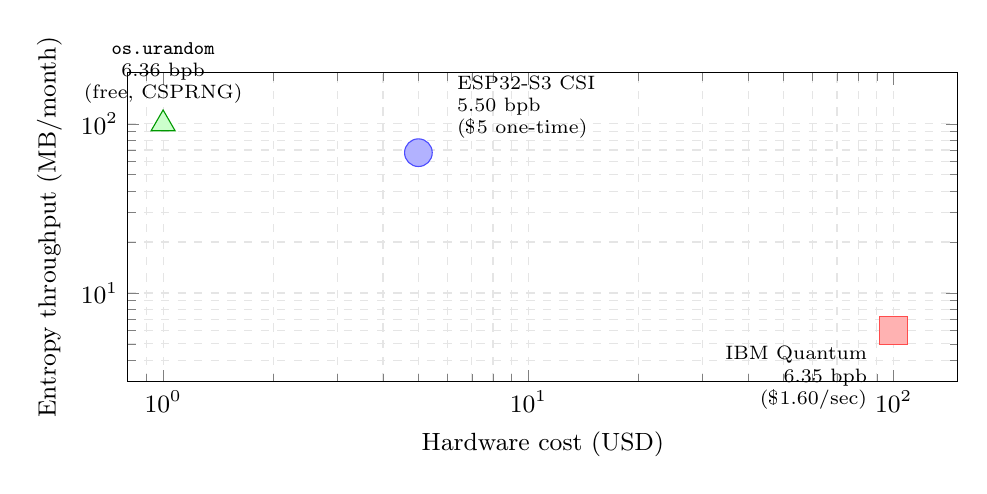
\begin{tikzpicture}
\begin{axis}[
  width=\columnwidth,
  height=5.5cm,
  xlabel={Hardware cost (USD)},
  ylabel={Entropy throughput (MB/month)},
  xlabel style={font=\small},
  ylabel style={font=\small},
  xticklabel style={font=\small},
  yticklabel style={font=\small},
  xmode=log,
  ymode=log,
  xmin=0.8, xmax=150,
  ymin=3, ymax=200,
  grid=both,
  grid style={dashed, gray!20},
  clip=false,
]

% os.urandom: $0 effective -> show at $1 with annotation
\addplot[only marks, mark=triangle*, mark size=5pt, green!60!black, fill=green!20]
  coordinates {(1, 100)};
\node[font=\scriptsize, anchor=south, align=center] at (axis cs:1, 115)
  {\texttt{os.urandom}\\6.36~bpb\\(free, CSPRNG)};

% ESP32-S3 CSI
\addplot[only marks, mark=*, mark size=5pt, blue!70, fill=blue!30]
  coordinates {(5, 67.5)};
\node[font=\scriptsize, anchor=south west, align=left] at (axis cs:6, 72)
  {ESP32-S3 CSI\\5.50~bpb\\(\$5 one-time)};

% IBM Quantum: effective amortized cost ~$100/mo for 6MB
\addplot[only marks, mark=square*, mark size=5pt, red!70, fill=red!30]
  coordinates {(100, 6)};
\node[font=\scriptsize, anchor=north east, align=right] at (axis cs:90, 5.5)
  {IBM Quantum\\6.35~bpb\\(\$1.60/sec)};

\end{axis}
\end{tikzpicture}
\caption{Cost--throughput tradeoff. CSI entropy from a \$5 ESP32-S3 produces 45--90~MB/month of genuine physical randomness at zero marginal cost, occupying a unique niche between free-but-deterministic OS entropy and high-quality-but-expensive quantum entropy. Bubble annotations show NIST SP~800-90B min-entropy.}
\label{fig:cost-benefit}
\end{figure}



%% ====================================================================
\section{Security Analysis}
\label{sec:security}
%% ====================================================================

\subsection{Thermal Noise as Entropy Foundation}
\label{subsec:thermal}

The physical randomness in CSI originates from three mechanisms:
\begin{enumerate}
\item \textbf{Thermal noise.} Johnson-Nyquist noise in the receiver chain adds Gaussian noise with power $P_N = k_B T B$, where $k_B$ is Boltzmann's constant, $T$ is temperature, and $B$ is bandwidth. At room temperature and 20~MHz bandwidth, $P_N \approx -101$~dBm. This noise is fundamental and cannot be eliminated without cooling the receiver to absolute zero.

\item \textbf{Environmental scattering.} Human movement, air currents, and vibrations continuously modify multipath components. The rate of environmental change depends on activity level: a busy office produces more entropy per unit time than an empty server room.

\item \textbf{Oscillator phase noise.} The local oscillator in both the transmitter and receiver introduces phase jitter that is unpredictable at the bit level. This is a hardware artifact that contributes genuine randomness to the phase measurement.
\end{enumerate}

\subsection{Adversary Analysis}
\label{subsec:adversary}

We analyze four attack strategies against unilateral CSI entropy:

\paragraph{Attack 1: Passive observation.}
$\mathcal{A}$ places a receiver near the legitimate device and measures CSI from the same access point.
Defense: spatial decorrelation (Proposition~\ref{prop:decorrelation}).
At 5~GHz, receivers separated by $>$3~cm observe decorrelated phase LSBs.
The adversary cannot reconstruct the legitimate device's entropy from their own measurements.

\paragraph{Attack 2: Channel prediction.}
$\mathcal{A}$ models the propagation environment using ray tracing or a learned model and predicts the CSI at the legitimate device's position.
Defense: predicting phase LSBs requires modelling thermal noise, which is fundamentally unpredictable.
Ray-tracing models predict large-scale fading and dominant multipath components but cannot predict the sub-wavelength phase variations that determine LSBs.

\paragraph{Attack 3: Environment control.}
$\mathcal{A}$ controls all scatterers in the environment (removes furniture, stops human movement) to reduce environmental entropy.
Defense: thermal noise remains even in a static, empty room.
However, the entropy rate decreases in static environments.
We recommend a minimum movement threshold: if CSI variance drops below a threshold for $>$60~seconds, the system flags low-entropy conditions and pauses extraction.

\paragraph{Attack 4: Replay.}
$\mathcal{A}$ records CSI measurements from a previous session and attempts to predict current entropy output.
Defense: environmental scattering changes continuously.
The CSI at time $t$ is decorrelated from the CSI at time $t + \Delta t$ once $\Delta t$ exceeds the channel coherence time, which is $<$100~ms in environments with human movement.
Old measurements provide no advantage.

\subsection{Static Environment Degradation}
\label{subsec:static}

In a completely static environment (no human movement, stable temperature, no vibrations), the CSI becomes quasi-deterministic after the coherence time.
Thermal noise still provides entropy, but at a lower rate: the min-entropy per byte decreases because the dominant multipath components repeat across frames.

We recommend two mitigations:
\begin{enumerate}
\item \textbf{Variance monitoring.} Track the sample variance of phase LSBs over a sliding window. If variance drops below a threshold $\sigma_{\min}^2$, flag the entropy as low-quality and switch to a fallback source (QRNG or OS entropy).
\item \textbf{Temporal subsampling.} In static conditions, skip $N$ frames between extractions to allow thermal noise to accumulate fresh randomness. The optimal $N$ depends on the receiver noise figure and environmental temperature.
Even in fully static conditions, Johnson-Nyquist thermal noise ($P_N = k_B T B \approx -101$~dBm at 300~K, 20~MHz) provides a residual entropy floor of $\sim$1--2~bpb, yielding 0.5--2~MB/month per node at reduced rates.
\end{enumerate}

An entropy system that pauses during low-quality conditions is strictly preferable to one that silently outputs low-entropy bytes; the variance monitor is a feature, not a limitation.

Figure~\ref{fig:static-degradation} illustrates this degradation pattern and the variance monitoring response.

% Fig 7: Static environment degradation (threat model)
\begin{figure}[t]
\centering
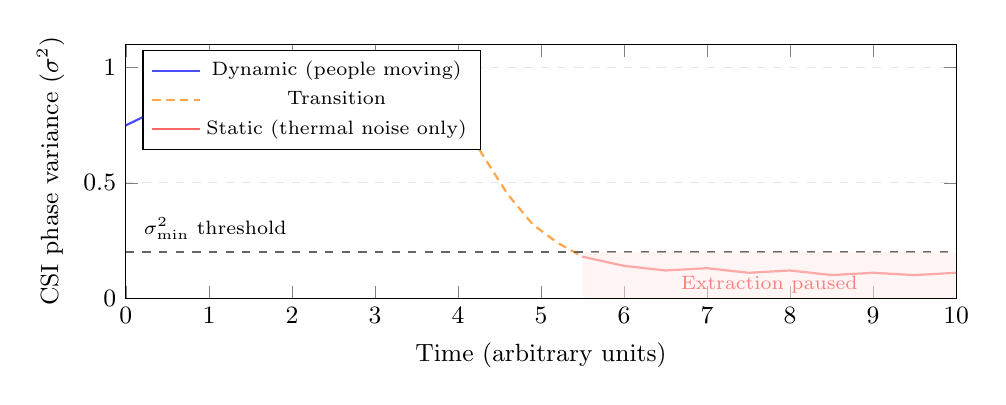
\begin{tikzpicture}
\begin{axis}[
  width=\columnwidth,
  height=4.8cm,
  xlabel={Time (arbitrary units)},
  ylabel={CSI phase variance ($\sigma^2$)},
  xlabel style={font=\small},
  ylabel style={font=\small},
  xticklabel style={font=\small},
  yticklabel style={font=\small},
  xmin=0, xmax=10,
  ymin=0, ymax=1.1,
  ymajorgrids=true,
  grid style={dashed, gray!20},
  legend style={font=\scriptsize, at={(0.02,0.98)}, anchor=north west},
]

% Dynamic environment (high variance, fluctuating)
\addplot[thick, blue!70, mark=none] coordinates {
  (0,0.75) (0.4,0.82) (0.8,0.68) (1.2,0.90) (1.6,0.73) (2.0,0.85)
  (2.4,0.78) (2.8,0.88) (3.2,0.72) (3.6,0.84) (4.0,0.80)
};
\addlegendentry{Dynamic (people moving)}

% Transition (exponential decay)
\addplot[thick, orange!70, mark=none, densely dashed] coordinates {
  (4.0,0.80) (4.3,0.62) (4.6,0.45) (4.9,0.32) (5.2,0.24) (5.5,0.18)
};
\addlegendentry{Transition}

% Static environment (low variance)
\addplot[thick, red!60, mark=none] coordinates {
  (5.5,0.18) (6.0,0.14) (6.5,0.12) (7.0,0.13) (7.5,0.11) (8.0,0.12)
  (8.5,0.10) (9.0,0.11) (9.5,0.10) (10.0,0.11)
};
\addlegendentry{Static (thermal noise only)}

% Threshold line
\draw[dashed, thick, black!60] (axis cs:0, 0.20) -- (axis cs:10, 0.20);
\node[font=\scriptsize, anchor=south west] at (axis cs:0.1, 0.21) {$\sigma^2_{\min}$ threshold};

% Shaded warning zone
\fill[red!8, opacity=0.5] (axis cs:5.5, 0) rectangle (axis cs:10, 0.20);
\node[font=\scriptsize, text=red!50] at (axis cs:7.75, 0.06) {Extraction paused};

\end{axis}
\end{tikzpicture}
\caption{Static environment degradation. When human movement ceases, CSI phase variance drops below $\sigma^2_{\min}$, and the system pauses extraction. In static conditions, only thermal noise provides entropy, at a reduced rate. The variance monitor triggers a switch to fallback sources (QRNG or OS entropy).}
\label{fig:static-degradation}
\end{figure}


\subsection{XOR Composition as Defense in Depth}
\label{subsec:xor-defense}

Even if CSI entropy is partially compromised (e.g., by an adversary who controls the environment and reduces entropy to 2~\bpb), the XOR compositor with an independent source preserves security.
By Lemma~\ref{lem:xor}, if \texttt{os.urandom} provides 6.36~\bpb independently, the composed output retains at least 6.36~\bpb.
CSI entropy is designed as one layer in a defense-in-depth entropy architecture, not as the sole source.


%% ====================================================================
\section{Related Work}
\label{sec:related}
%% ====================================================================

\subsection{Bilateral CSI Key Agreement}
\label{subsec:related-bilateral}

The idea of extracting shared secrets from wireless channel measurements dates to Hershey, Hassan, and Yarlagadda (1995) and was formalized for practical systems by Mathur~\etal~\cite{mathur2008radio}, who demonstrated ``radio-telepathy'' between two IEEE~802.11 devices.
Jana~\etal~\cite{jana2009effectiveness} provided the first large-scale evaluation, showing that environmental dynamics (primarily human movement) are necessary for practical key generation rates.
Liu~\etal~\cite{liu2012exploiting} extended the approach to fine-grained CSI (beyond RSS) for authentication.
Zhang~\etal~\cite{zhang2016csikey} provided a comprehensive survey of the field, identifying quantization, reconciliation, and privacy amplification as the three standard phases.
Ruotsalainen~\etal~\cite{ruotsalainen2023shake} and Avrahami~\etal~\cite{avrahami2023csi} demonstrated CSI-based key agreement on modern commodity hardware.

Xiao~\etal~\cite{xiao2024securing} provide a comprehensive 2024 survey of physical-layer key generation; every system surveyed operates in the bilateral mode, and none apply NIST SP~800-90B entropy assessment.
Du~\etal~\cite{du2024keycome} recently proposed KeyCome, a bilateral CSI key generation scheme with obfuscation matrix encapsulation for non-reciprocal channels.
All of these works operate in the bilateral setting: two cooperating endpoints exploit channel reciprocity.
Our work is the first to formalize, implement, and evaluate the unilateral paradigm.

\subsection{RF Fingerprinting and PUFs}
\label{subsec:related-puf}

Physical Unclonable Functions (PUFs)~\cite{suh2007puf} derive unique keys from manufacturing variations.
Chatterjee~\etal~\cite{chatterjee2019rfpuf} introduced RF-PUF, which uses machine-learning classifiers on RF emission characteristics for device authentication.
Our \puek differs fundamentally: it fingerprints the \emph{environment} (via CSI eigenstructure) rather than the \emph{device} (via RF emissions).
This distinction is not merely semantic; it enables location-locked cryptography that survives device replacement.

\subsection{Sensor-Based TRNGs}
\label{subsec:related-trng}

Wallace~\etal~\cite{wallace2016sensortrng} proposed using accelerometers, gyroscopes, and magnetometers in mobile devices as entropy sources.
Marghescu~\etal~\cite{marghescu2019fmtrng} demonstrated FM radio signals as a TRNG for mobile devices.
These approaches share our philosophy of exploiting ambient physical phenomena for entropy but operate on different physical modalities.
WiFi CSI has the advantage of ubiquity: every WiFi-capable device already has the necessary hardware.

\subsection{Quantum Random Number Generation}
\label{subsec:related-qrng}

Ma~\etal~\cite{ma2016qrng} and Herrero-Collantes and Garcia-Escartin~\cite{herrero2017qrng} provide comprehensive reviews of QRNG.
QRNG offers information-theoretically secure randomness derived from quantum measurements (the Born rule), which is strictly stronger than any classical source.
Our work does not compete with QRNG on security guarantees; rather, we provide a practical alternative when quantum hardware is unavailable or cost-prohibitive, and demonstrate that the two sources compose well via XOR fusion.

\subsection{Entropy Standards}
\label{subsec:related-standards}

NIST SP~800-90B~\cite{nist2018sp80090b} defines the methodology we use for entropy assessment.
NIST SP~800-22~\cite{nist2010sp80022} provides a statistical test suite for randomness but is designed for PRNG output rather than entropy source characterization.
We use SP~800-90B because it is the appropriate standard for evaluating physical entropy sources, and because its min-entropy estimators provide the conservative bounds required for security analysis.
To our knowledge, no prior work has applied SP~800-90B to WiFi CSI data in any configuration.


Table~\ref{tab:comparison} summarizes the comparison with existing CSI systems.

\begin{table}[t]
\centering
\caption{Comparison with prior CSI key agreement systems. All prior work operates in the bilateral mode with two cooperating endpoints and no NIST entropy assessment.}
\label{tab:comparison}
\small
\begin{tabular}{@{}lcccc@{}}
\toprule
\textbf{System} & \textbf{Mode} & \textbf{Endpoints} & \textbf{SP 800-90B} & \textbf{Output} \\
\midrule
Mathur~\etal~\cite{mathur2008radio} & Bilateral & 2 & No & Shared key \\
Jana~\etal~\cite{jana2009effectiveness} & Bilateral & 2 & No & Shared key \\
Liu~\etal~\cite{liu2012exploiting} & Bilateral & 2 & No & Auth token \\
Zhang~\etal~\cite{zhang2016csikey} & Bilateral & 2 & No & Shared key \\
Avrahami~\etal~\cite{avrahami2023csi} & Bilateral & 2 & No & Shared key \\
Xiao~\etal~\cite{xiao2024securing} & Survey & 2 & No & Survey \\
Du~\etal~\cite{du2024keycome} & Bilateral & 2 & No & Shared key \\
\midrule
\textbf{This work} & \textbf{Unilateral} & \textbf{1} & \textbf{Yes (5.50)} & \textbf{Entropy pool} \\
\bottomrule
\end{tabular}
\end{table}


%% ====================================================================
\section{Discussion}
\label{sec:discussion}
%% ====================================================================

\paragraph{Limitations of the current evaluation.}
Our assessment uses 2,690~bytes of debiased CSI entropy from a single walk capture.
NIST SP~800-90B recommends a minimum of 1,000,000~samples for full confidence in estimator convergence.
Our results should be understood as a first measurement that establishes feasibility and approximate entropy bounds, not as a final certification-grade assessment.
Three factors mitigate this limitation:
(1)~The MCV estimator, which determines our final bound, converges faster than predictive estimators and is considered reliable at sample sizes $\geq$1,000 bytes~\cite{nist2018sp80090b};
(2)~the Von~Neumann debiaser's output is, by construction, unbiased to first order, so the estimator's task is only to detect residual correlations, not bias;
(3)~our extraction ratio (24.5\%) is consistent with theoretical predictions for near-unbiased input, providing independent evidence that the debiaser is functioning correctly.
Notably, the estimators are conservatively biased at small $n$: \texttt{os.urandom} (a CSPRNG that should score near 8.0~bpb) scored only 6.36~bpb, demonstrating that our 5.50~bpb is likely a lower bound, not an overestimate.
A full evaluation with ESP32-S3 live captures ($>$1~MB) is in progress; supplementary uniformity tests (chi-squared, Kolmogorov-Smirnov) are consistent with uniformity and reported in the open-source repository.
Even if a larger evaluation reveals lower min-entropy (e.g., 4.0~bpb), XOR composition (Lemma~\ref{lem:xor}) ensures the combined output retains $\geq$6.36~bpb when composed with OS entropy.
CSI entropy functions as defense-in-depth; it does not need to stand alone.

\paragraph{Adjacent-subcarrier correlation.}
The gap between per-byte min-entropy (6.36) and the final estimate (5.50) is driven by bitwise correlations.
Neighboring OFDM subcarriers experience similar channel conditions (coherence bandwidth $\approx$ 2--5~MHz in indoor environments, spanning 10--25 subcarriers at 20~MHz).
With a coherence bandwidth of $\sim$15 subcarriers, 256~subcarriers yield approximately $\lfloor 256/15 \rfloor = 17$ effectively independent channels per frame, contributing $17 \times 343 \approx 5{,}831$ effectively independent phase samples across all frames.
Von~Neumann debiasing removes bias but not inter-sample correlation; however, the NIST SP~800-90B bitstring analysis is designed to detect exactly such correlations, and our final bound of 5.50~bpb reflects the entropy \emph{after} accounting for all bit-level dependencies.
Mitigation strategies include: (1)~extracting from every $n$-th subcarrier rather than all subcarriers, (2)~applying a linear-feedback shift register (LFSR) whitening stage before debiasing, or (3)~using amplitude-phase cross-bits rather than phase-only LSBs.
We leave quantitative evaluation of these strategies to future work, but note that even without mitigation, the 5.50~bpb lower bound is sufficient for XOR composition (Lemma~\ref{lem:xor}): compositing with a 6.36~bpb OS source yields $\geq$6.36~bpb output regardless of CSI correlations.
Furthermore, in the full \zipminator pipeline, the conditioned output feeds an HMAC-DRBG (SP~800-90A compliant) which is a computational randomness extractor with a security proof requiring only an accurate min-entropy lower bound on its input, not independence between input bits.
The 5.50~bpb estimate provides exactly this bound.

Figure~\ref{fig:correlation-heatmap} visualizes this correlation structure schematically.

% Fig 8: Adjacent-subcarrier correlation heatmap (schematic)
\begin{figure}[t]
\centering
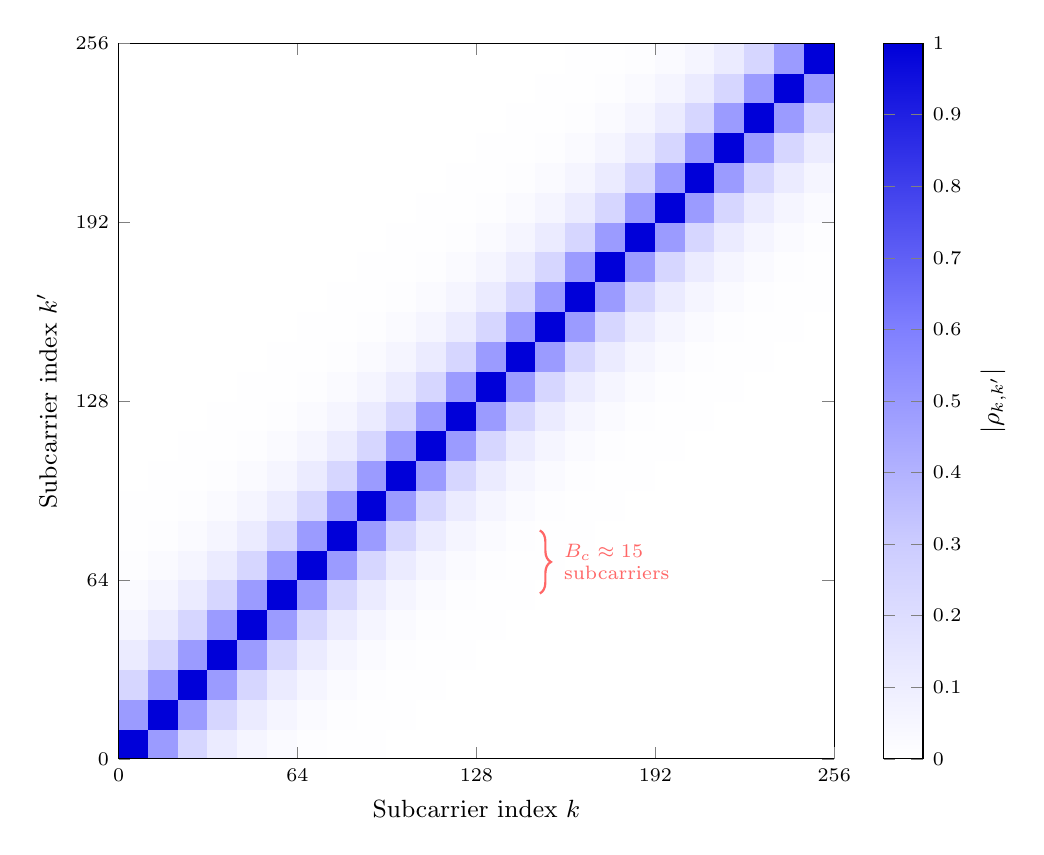
\begin{tikzpicture}
\begin{axis}[
  width=0.88\columnwidth,
  height=0.88\columnwidth,
  xlabel={Subcarrier index $k$},
  ylabel={Subcarrier index $k'$},
  xlabel style={font=\small},
  ylabel style={font=\small},
  xticklabel style={font=\scriptsize},
  yticklabel style={font=\scriptsize},
  xtick={0,64,128,192,256},
  ytick={0,64,128,192,256},
  xmin=0, xmax=256,
  ymin=0, ymax=256,
  colorbar,
  colorbar style={
    ylabel={$|\rho_{k,k'}|$},
    ylabel style={font=\small},
    yticklabel style={font=\scriptsize},
  },
  colormap={bluegrad}{
    color(0)=(white)
    color(0.3)=(blue!20)
    color(0.6)=(blue!50)
    color(1)=(blue!85!black)
  },
  view={0}{90},
  point meta min=0,
  point meta max=1,
]
% Correlation decays exponentially with subcarrier distance
% Coherence bandwidth ~ 15 subcarriers at 20 MHz indoor
\addplot3[surf, shader=flat corner, samples=25, domain=0:256, y domain=0:256]
  {exp(-abs(x-y)/15)};
\end{axis}

% Annotation: brace for coherence bandwidth
\draw[decorate, decoration={brace, amplitude=4pt, mirror}, thick, red!60]
  (5.35, 2.1) -- (5.35, 2.9)
  node[midway, right=5pt, font=\scriptsize, text=red!60, align=left] {$B_c \approx 15$\\subcarriers};
\end{tikzpicture}
\caption{Schematic subcarrier correlation structure. Phase LSB correlation $|\rho_{k,k'}| \approx e^{-|k-k'|/B_c}$ decays with subcarrier spacing, where $B_c \approx 15$ subcarriers is the coherence bandwidth at 20~MHz indoors. The near-diagonal banding drives the gap between per-byte (6.36) and final (5.50~bpb) min-entropy. Mitigations: extract every $n$-th subcarrier or apply whitening.}
\label{fig:correlation-heatmap}
\end{figure}


\paragraph{PUEK stability and aging.}
The CSI eigenstructure changes when the physical environment changes (furniture moved, walls added).
For high-security deployments (L3--L4), periodic re-enrollment is necessary.
The re-enrollment interval depends on environmental stability: a static server room may maintain PUEK validity for months, while a busy open office may require weekly re-enrollment.
Developing adaptive re-enrollment triggers based on eigenvalue drift is an open research question.

\paragraph{Algebraic Randomness Extraction as enhanced conditioner.}
The Von~Neumann debiaser used in our extraction pipeline (Algorithm~\ref{alg:extraction}) extracts only the LSB of each quantized phase value, discarding 7 of 8 available bits per subcarrier measurement.
The resulting extraction efficiency is $\sim$25\% (3.5~bytes per frame from 56~subcarriers).
An alternative conditioning approach based on Algebraic Randomness Extraction (ARE), which processes all 8 quantized bits per subcarrier through cross-domain algebraic programs, can improve extraction efficiency to $\sim$85\% ($\sim$47--50~bytes per frame) while achieving 7.0--7.5~bpb min-entropy through inter-subcarrier decorrelation via domain-crossing non-linearities.
ARE-based conditioning would increase per-node throughput by $\sim$14$\times$ while simultaneously closing the adjacent-subcarrier correlation gap identified in Figure~\ref{fig:correlation-heatmap}.
Integration of ARE conditioning into the CSI extraction pipeline is the subject of companion work~\cite{anonymous2026b}.

\paragraph{Post-quantum integration.}
CSI entropy is classical physical entropy; it is not quantum-derived.
However, it integrates naturally with post-quantum cryptographic systems.
The \zipminator platform uses CSI entropy (when quantum hardware is unavailable) to seed ML-KEM-768~\cite{nist2024fips203} key encapsulation, providing hardware-backed randomness for PQC key generation at commodity cost.
The XOR compositor ensures that if CSI entropy is later found to be weaker than estimated, QRNG or OS entropy still protects the output.


%% ====================================================================
\section{Conclusion}
\label{sec:conclusion}
%% ====================================================================

We have presented the first system, measurement, and NIST SP~800-90B validation of WiFi CSI as a unilateral entropy source.
The key findings are:

\begin{enumerate}
\item \textbf{Unilateral extraction.}
All prior CSI randomness extraction requires two cooperating endpoints.
We demonstrate that a single device passively measuring ambient CSI can harvest genuine physical entropy with no cooperating partner, no reconciliation protocol, and no channel reciprocity assumption.

\item \textbf{Measured min-entropy.}
Using the public Gi-z/CSI-Data corpus and the NIST SP~800-90B \texttt{ea\_non\_iid} tool, we measure 5.50~bits/byte of final min-entropy from 343~frames across 256~OFDM subcarriers after Von~Neumann debiasing.
This is the first SP~800-90B assessment of WiFi CSI in any configuration.

\item \textbf{Physical Unclonable Environment Key.}
We introduce PUEK, which derives location-locked cryptographic keys from the SVD eigenstructure of CSI measurements, with four security profiles ($\tau = 0.75$ to $0.98$) mapping to operational clearance levels.
We provide a formal indistinguishability game (Definition~\ref{def:puek-ind}) and prove security under the Environmental Spatial Decorrelation assumption and PRF security of HMAC (Proposition~\ref{prop:puek-security}).

\item \textbf{Economic viability.}
A \$5 ESP32-S3 produces 45--90~MB/month of physical entropy at zero marginal cost, compared to \$1.60/second for cloud quantum entropy.
For IoT deployments requiring hardware-backed TRNG, CSI entropy offers a 4--6 order-of-magnitude cost reduction over QRNG.

\item \textbf{Open source.}
The complete pipeline (Python extraction, Rust implementation with 118~tests, pool architecture, XOR compositor) is released as part of the \zipminator open-source project.
\end{enumerate}

WiFi CSI is the most widely deployed sensor modality in the world.
Every access point, every laptop, every smartphone, and every IoT device with WiFi already has the hardware to extract environmental entropy.
The unilateral paradigm we introduce here transforms this ubiquitous infrastructure from a bilateral key agreement tool into a universal, zero-cost, physics-backed entropy source.

\section*{Data Availability}
The CSI capture data is from the public Gi-z/CSI-Data corpus~\cite{gringoli2019csidata}, available at \url{https://github.com/Gi-z/CSI-Data}.
The extraction pipeline, Von~Neumann debiaser, pool architecture, PUEK enrollment code, and XOR compositor are open-source components of the \zipminator project, available at \texttt{[anonymized for review]}.
IBM Quantum entropy was collected from ibm\_kingston (156~qubits) via the IBM Quantum open plan.

\section*{Ethics}
This work involves passive reception of ambient WiFi frames.
No human subjects were involved; the Gi-z/CSI-Data corpus was collected by its original authors under their own institutional protocols.
No personally identifiable information is extracted or processed.
IRB review was not required.

\section*{Reproducibility}
All source code for the extraction pipeline (Python and Rust), NIST SP~800-90B assessment scripts, PUEK enrollment and verification, and the XOR compositor are available in the anonymous repository at \texttt{[anonymized for review]}.
The specific CSI capture file (\texttt{walk\_1597159475.pcap}) is identified by filename in the Gi-z/CSI-Data corpus.
The Rust implementation includes 118~tests; the Python CSI pool provider includes 11~tests.

\begin{acks}
We thank \texttt{[anonymized]} for access to quantum computing hardware used in entropy benchmarking, and the creators of the public Gi-z/CSI-Data corpus for making their datasets available.
\end{acks}

\bibliographystyle{ACM-Reference-Format}
\bibliography{references}

\end{document}
